\nocite{ddd_eric_evans}
\nocite{gof_patterns}
\nocite{sonda_project}
\nocite{nosql_distilled}
\nocite{js_async}

\chapter{Introdução}

A captação de energia elétrica no Brasil, é composta por diversas fontes primárias, dentre as quais, se destacam o uso de energia eólica, energia hidráulica e energia solar, dentre as tais, a energia solar de destaca por sua baixa implicação a questões ambientais.

A energia solar, vem sendo cada vez mais amplamente utilizada utilizada no Brasil, tanto por empresas de pequeno a grande porte, quanto pelo mercado residencial, segundo a projeção da Associação Brasileira de Energia Solar Fotovoltaica (Absolar), tal forma de captação de energia representa 0,83\% de toda a energia captada no país \cite{maturidade_absolar}.

Mesmo com o amadurecimento da captação de energia solar no país, o projeto de instalação de uma estação de captura de energia solar, necessita ser feito juntamente com uma prévia análise de dados no local, para que, resultados satisfatórios possam ser obtidos a mínimo prazo.

O trabalho desenvolvido visa fornecer uma ferramenta para a captura e análise de dados meteorológicos, visando a geração de informações necessárias para o usuário.

\section{Objetivo}

O trabalho tem como objetivo fornecer uma ferramenta para captura, persistência e análise de dados meteorológicos, fornecendo a usuários, informações necessárias para o acompanhamento da eficiência energética de painéis solares.

Aproveitando-se do baixo custo de equipamentos eletrônicos para disponibilizar um software como um todo de baixo custo e de fácil instalação.

Para se atingir o objetivo especificado, foi construído um software de amostragem de dados ao usuário, realizando previamente um tratamento e análise de dados.

\section{Justificativa}

A justificativa do desenvolvimento do trabalho se da pela iniciativa da instalação de uma usina solar no Instituto Federal de São Paulo, no Campus localizado em Boituva.

Foi implementado um laboratório de 30$m^2$, composto por uma estação solarimétrica e um sistema de 5$kW$ com rastreador solar, entre outras tecnologias.

O projeto de exploração de energia fotovoltaica proporcionou a criação do curso de instalador de sistemas fotovoltaicos, onde a ferramenta visa ser utilizada de forma a agrupar os dados capturados em diferentes pontos \cite{solar_ifsp_btv}.

\section{Estrutura do TCC}

O trabalho apresentado, primeiramente procura contextualizar acerca da atual situação da captação de energia solar, procurando explicar conceitos básicos de energia fotovoltaica e decorre sobre as dificuldades e cuidados entorno do assunto.

Subseguindo, são apresentadas as metodologias utilizadas no desenvolvimento do projeto, decorrendo acerca das ferramentas utilizadas e conceitos nos quais o projeto se baseia, no desenvolvimento do trabalho, em seguida, é apresentado ao usuário o projeto do sistema, onde questões teóricas acerca da implementação são discutidas, seguindo o desenvolvimento do projeto, se apresenta a arquitetura e documentação do software, detalhando questões internas do desenvolvimento do software e as justificativas pelas tecnologias utilizadas.

Por fim, são apresentadas as considerações finais do projeto, demonstrando os resultados obtidos, comparando os mesmos com os requisitos, procurando esclarecer os objetivos atingidos ou não, e então, é feita uma projeção do projeto para o futuro, apresentando um caminho para o projeto de manutenção e continuidade do software.

\chapter{Referencial Teórico}

TODO: REFERENCIAL TEORICO

\chapter{Desenvolvimento}

\section{Metodologias}

\subsection{Programação funcional}

Foi utilizado para a elaboração da arquitetura do software, conceitos de programação funcional, sua maior característica é que, se uma expressão possui um valor bem definido, então, dada uma entrada de dados, a ordem a qual o computador carregar a avaliação não afeta o resultado \cite{introduction_functional}.

A programação funcional, visa, através da utilização do conceito matemático de funções, proporcionar para a arquitetura do software, um modelo onde funções recebem parâmetros e então, através dos parâmetros que foram inseridos na função, um valor é sempre retornado para este parâmetro, este conceito é chamado de função pura, uma vez que um valor $x$ é colocado com entrada, sempre se terá como resposta o valor y. Através das funções puras, o código se torna mais previsível e mais suscetível a testes automatizados, fazendo comparação com o paradigma de programação orientada a objetos, muitas vezes, o objeto está em um estado inválido na memória, podendo assim, acarretar erros.

Porém, nem sempre o controle de estado colateral é levado como lei, porém, ele é contido dentro de funções que estão encapsuladas em locais específicos da aplicação, desta forma, o risco de erros diminui, visando a alta disponibilidade do sistema, que, agora, não depende mais de uma alta quantidade de contextos externos.

\subsection{Controle de qualidade}

Foram utilizadas, juntamente ao desenvolvimento do software, técnicas de controle de software orientadas ao teste, onde, a aplicação é submetida a seção de testes, tanto manuais como automatizados, foram utilizados testes de interface no sistema e testes unitários automatizados.

\subsubsection{Testes de interface}

Para que fosse validada a funcionalidade do sistema como um todo, testes de interface no sistema foram aplicados, onde, diversos usuários foram submetidos a utilização do sistema, informando possíveis dificuldades na utilização do mesmo e erros, que, uma vez corrigidos, voltam a serem analisados por usuários, até que se possa ser atingida uma mínima aceitação.

\subsubsection{Testes unitários}

Segundo \citeauthoronline{tdd_by_example}, (\citeyear{tdd_by_example}, p.10), "Desenvolvimento orientado a testes, é uma maneira de gerenciar o medo durante a programação".

O conceito de testes unitários em desenvolvimento de software, é fornecer a uma unidade, que pode ser considerada como uma função ou uma instrução do sistema, valores esperados, valores esses, que são comparados com os retornos das funções, e que, uma vez não correspondendo, emitem um erro ao desenvolvedor, que pode, com a visualização facilitada do problema, corrigir tal ponto de forma acertiva.

Tal conceito fora aplicado, para garantir, de forma unitária a qualidade e segurança do código fonte do sistema, garantindo assim, a qualidade da aplicação, desde os primeiros momentos de sua implementação.

\subsection{Diagramas UML 2.0}

Assim como definido por \citeauthoronline{uml_pratica}, (\citeyear{uml_pratica}), a UML:

\begin{citacao}
    É uma linguagem utilizada para modelar softwares baseados no paradigma de orientação a objetos. É uma linguagem de modelagem de propósito geral que pode ser aplicada a todos os domínios de aplicação. (p.17).
\end{citacao}

No trabalho apresentado, mesmo que não utilizados conceitos de orientação a objetos, a linguagem de modelagem UML foi utilizada como ferramenta para detalhar partes do software, descrevendo desde os casos de uso da aplicação, as funcionalidades do sistema.

\section{Ferramentas utilizadas}

\subsection{Astah}

Astah Community é um software para modelagem UML com suporte a UML 2, desenvolvido pela Change Vision, e disponível para diversos sistemas operacionais. Anteriormente conhecido por JUDE, um acrônimo de Java and UML Developers Environment (Ambiente para Desenvolvedores UML e Java) \cite{astah_uml}.

O mesmo foi utilizado no projeto para a criação dos diagramas de descrição software, auxiliando no desenho dos casos de uso na engenharia de requisitos e nos diagramas de classe, diagramas de sequência, estado e implementação.

A utilização do software Astah, foi motivada pela sua confiabilidade na construção dos diagramas, fornecendo uma plataforma com redundâncias e por fornecer uma licença gratuita de sua versão profissional a universidades e estudantes de engenharia de software.

\subsection{Javascript ES8}

O Javascript é um linguagem de programação interpretada multiparadigma, aceitando estilos variados de programação como orientação a objetos, programação funcional e imperativa \cite{mozilla_javascript}. O Javascript é uma linguagem de programação primariamente desenvolvida para o lado do cliente, sendo executada no navegador do usuário, porém, com o advento do motor de processamento do motor do Google Chrome, o v8, a linguagem foi implementada também do lado servidor, utilizando o motor de processamento nodejs, que é baseada no motor do Chrome \cite{nodejs_about}.

Para a implementação do projeto, foi utilizada a linguagem de programação Javascript em sua versão 8, ou como definida pela especificação do Javascript, o EcmaScript 2017.

A utilização da linguagem Javascript, tanto para a construção da aplicação no lado servidor, quando para o lado cliente, foi determinada por sua alta performance e por proporcionar ferramentas que permitem a programação de forma funcional, detalhes acerca da utilização da linguagem são melhor definidos na seção acerca dos detalhes da implementação do software, em \ref{sec:arquitetura_software}.

\subsection{MongoDB}

O MongoDB é um banco de dados de documento com suporte a escalabilidade e flexibilidade para execução de consultas e indexação necessária \cite{what_mongodb}.

O mesmo foi utilizado no projeto em sua versão 4.1, a justificativa de seu uso, se da pela sua facilidade ao se trabalhar com escrita massiva de informações, proporcionando a aplicação performance e disponibilidade.

\section{Engenharia de requisitos}

Assim como descrito por \citeauthoronline{engenharia_software_pressman} (\citeyear{engenharia_software_pressman}):

\begin{citacao}
O amplo espectro de tarefas e técnicas que levam a um entendimento dos requisitos é denominado engenharia de requisitos. Na perspectiva do processo de software, a engenharia de requisitos é uma ação de engenharia de software importante que se inicia durante a atividade de comunicação e continua na de modelagem. Ela deve ser adaptada às necessidades do processo, do projeto, do produto e das pessoas que estão realizando o trabalho. (p.126).
\end{citacao}

Neste capítulo, há a utilização da engenharia de requisitos para auxiliar a documentação do projeto de software, descrevendo os cenários de utilização de sistema, onde é descrito o comportamento esperado pelo usuário através de entrevistas, após, utilizando os resultados obtidos com a modelagem através de cenários, os requisitos são definidos e são criados os contratos de uso do usuário com o sistema através de casos de uso, então, é descrita a arquitetura macro do software, procurando contextualizar acerca do desenho do projeto.

\subsection{Cenários do sistema}

Há diversas formas de se medir a qualidade de um software, porém, não há outra forma de se medir a qualidade e se um objetivo foi atingido no desenvolvimento de um sistema do que a satisfação dos usuários. Se entendido como os usuários desejam interagir com o sistema, o que é esperado de entradas, processamentos e saídas, será possível a equipe construir um projeto mais objetivo e proveitoso \cite{engenharia_software_pressman}. 

Portanto, nesta seção são descritos os cenários do software através de uma descrição que foi construída utilizando conteúdos das entrevistas que foram feitas com as partes interessadas no projeto.

No Instituto Federal de São Paulo, no campus localizado em Boituva, o professor responsável pelo projeto descreve o sistema como uma aplicação capaz de capturar dados meteorológicos através de sensores próximos a painéis solares, ele necessita dessas informações sendo demonstradas através de gráficos, para que uma análise possa ser feita, além da disposição das informações através de gráficos, é esperado do sistema demonstrar ao usuário informações de mínimas e máximas das informações capturadas. É desejado pelo usuário que o sistema seja capaz de lidar com diversas estações meteorológicas, reunindo os dados, portando, o sistema necessita de um cadastro das estações meteorológicas, guardando informações e identificações.

Através do texto acima, podemos entender as necessidades do usuário para com o sistema, o cenário de software descrito é definido dentro dos requisitos nas seções seguintes.

\subsection{Requisitos funcionais}

Os requisitos funcionais de um software são utilizados para descrever o que ele deve fazer, eles giram em torno do tipo de sistema desenvolvido, de seus usuários e da forma como uma equipe de desenvolvimento de software busca entender o que é necessário para criar um software que atenda as necessidades de um usuário. Ao serem descritas as funcionalidades básicas de um sistema, a fazemos de forma abstrata, para que os interessados no desenvolvimento do projeto possam entender o que será feito. Porém, os mesmos podem ser detalhados de forma especifica, declarando suas entradas, saídas e exceções \cite{engenharia_software_sommerville}.

Foi utilizado para descrever os requisitos funcionais do sistema, a modelagem de requisitos através do diagrama de caso de uso, que busca visualizar, especificar e documentar o comportamento de um ator ao utilizar o sistema. \cite{uml_pratica}.

O diagrama de caso de uso descrito na figura \ref{fig:figure_diagrama_caso_uso}, resume os requisitos funcionais que foram definidos ao longo do desenvolvimento do projeto.

\begin{figure}[H]
    \centering
    \caption{Diagrama de caso de uso} \label{fig:figure_diagrama_caso_uso}
    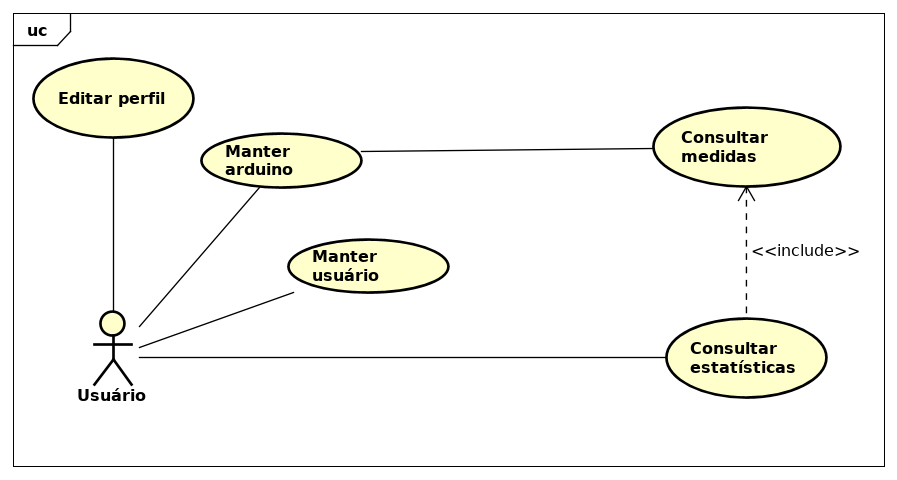
\includegraphics[scale=0.6]{diagrams/caso_de_uso.png}
    \hfill
\end{figure}

Através do diagrama do caso de uso contido na figura \ref{fig:figure_diagrama_caso_uso}, é possível identificarmos apenas um ator na aplicação, que é o usuário do sistema, interessado em visualizar informações geradas pela análise estatística dos dados capturados. O mesmo interage com a aplicação através da interface de usuário, realizando cadastros e consultas.

O requisito funcional \textbf{Consultar estatísticas} é o principal requisito do sistema, onde o usuário fará a filtragem dos dados, trazendo a ele as estatísticas geradas pela aplicação.
O usuário irá utilizar de campos de entrada de dados para escolher qual a estação meteorológica ele deseja visualizar, a data inicial para realizar as consultas, a data final e o intervalo de tempo para cálculo das médias.
Após a consulta das informações, o usuário irá obter como resultado as informações de mínimas e máximas das medidas e gráficos que o informam as médias para cada uma das propriedades meteorológicas.

O requisito funcional representado pelo caso de uso \textbf{Manter usuário}, descreve as ações do usuário acerca do cadastro de usuários no sistema.
Através desta funcionalidade, o usuário poderá, através da interface do usuário na web, utilizando tabelas, realizar o cadastro, consultas, atualização de informações e exclusão de usuários.
Durante a interação do usuário com a persistência de dados de usuários no sistema, caso erros ocorram, mensagens de erro auxiliares serão mostradas ao usuário, o auxiliando a encontrar qual o erro no processo realizado.

O requisito funcional \textbf{Manter arduino}, é muito similiar ao caso de uso anterior \textbf{Manter usuário}, e representa a persistência de informações acerca das estações meteorológicas no sistema, utilizando as quatro operações básicas de cadastro, consulta, atualização e exclusão de dados.

O requisito funcional de representado pelo caso de uso \textbf{Editar Perfil} representa a visualização e edição dos dados do usuário que está utilizando o sistema no momento, ele pode escolher editar suas informações, que exibe um formulário com os atuais dados preenchidos, onde o usuário pode realizar a alteração de suas informações.

\subsubsection{Detalhamento dos casos de uso}

Utilizando de tabelas, este capítulo descreve de forma detalhada cada um dos casos de uso, apresentado as descrições, os atores relacionados, as pré condições, exceções e fluxos alternativos.

\begin{table}[H]
    \ABNTEXfontereduzida
    \caption{Consultar estatísticas}
    \label{table:usecase_consultar_estatisticas}
    \begin{tabular}{{l}|p{10.5cm}}

    \hline

    \multicolumn{2}{c}{\textbf{Realizar consultas com filtros}} \\

    \hline
    Descrição & Recebe do usuário os filtros para seleção das informações, então, realiza uma análise estatística dos dados requisitados e os exibe para o usuário utilizando listagens e gráficos. \\

    \hline

    Atores & Usuário \\

    \hline

    \multirow{3}{*}{Pré-condições} & Banco de dados em correto funcionamento \\
    & Filtros corretos passados pelo usuário \\
    & Listagem de estações meteorológicas retornando ao mínimo uma estação \\

    \hline

    \multirow{2}{*}{Exceções e fluxos alternativos} & Caso a seleção não retorne nenhuma informação ao usuário, uma mensagem de dados inexistentes é exibida \\
    & Em caso de perca de conexão com banco de dados, exibe uma mensagem de erro ao usuário \\
    & Caso não existam estações meteorológicas cadastradas, o filtro de seleção de estação meteorológica exibe um aviso ao usuário \\

    \hline

    \end{tabular}
\end{table}

\begin{table}[H]
    \ABNTEXfontereduzida
    \caption{Especificações do caso de uso consultar medidas}
    \label{my-label}
    \begin{tabular}{{l}|p{10.5cm}}

    \hline

    \multicolumn{2}{c}{\textbf{Consultar medidas}} \\

    \hline
    Descrição & Consulta as medidas que estão persistidas no banco de dados para uma estação meteorológica, no software desenvolvido, atualmente este caso de uso é apenas acessado pela geração de estatísticas \\

    \hline

    \multirow{2}{*}{Pré-condições} & Credenciais de acesso ao banco de dados  \\
    & Banco de dados em correto funcionamento \\

    \hline

    \multirow{2}{*}{Exceções e fluxos alternativos} & Caso não existam medidas capturadas para a estação meteorológica, retorna uma lista vazia de dados \\

    \end{tabular}
\end{table}

\begin{table}[H]
    \ABNTEXfontereduzida
    \caption{Especificação do caso de uso manter usuários}
    \label{my-label}
    \begin{tabular}{{l}|p{10.5cm}}

    \hline

    \multicolumn{2}{c}{\textbf{Manter usuários}} \\

    \hline
    Descrição & Realiza uma listagem dos dados dos usuários atualmente registrados no sistema, fornecendo a possibilidade de cadastrar um novo usuário, atualizar os dados de um usuário ou excluir um usuário do sistema \\

    \hline

    \multirow{2}{*}{Pré-condições} & Credenciais de acesso ao banco de dados \\
    & Banco de dados em correto funcionamento \\

    \hline

    \multirow{2}{*}{Exceções e fluxos alternativos} & Caso não existam usuários cadastrados no sistema, exibe uma mensagem de aviso ao usuário \\
    & Para o cadastro ou atualização dos dados de um usuário, caso existam dados inválidos que foram dados como entrada, ao confirmar a operação, exibe uma mensagem de erro ao usuário \\

    \end{tabular}
\end{table}

\begin{table}[H]
    \ABNTEXfontereduzida
    \caption{Especificação do caso de uso manter estações meteorológicas}
    \label{my-label}
    \begin{tabular}{{l}|p{10.5cm}}

    \hline

    \multicolumn{2}{c}{\textbf{Manter estações meteorológicas}} \\

    \hline
    Descrição & Realiza uma listagem dos dados das estações meteorológicas atualmente registradas no sistema, fornecendo a possibilidade de cadastrar uma nova estação, atualizar os dados de uma estação ou excluir uma estação meteorológica do sistema \\

    \hline

    \multirow{2}{*}{Pré-condições} & Credenciais de acesso ao banco de dados  \\
    & Banco de dados em correto funcionamento \\

    \hline

    \multirow{2}{*}{Exceções e fluxos alternativos} & Caso não existam estações cadastradas no sistema, exibe uma mensagem de aviso ao usuário \\
    & Para o cadastro ou atualização dos dados de uma estação, caso existam dados inválidos que foram dados como entrada, ao confirmar a operação, exibe uma mensagem de erro ao usuário \\

    \end{tabular}
\end{table}

\begin{table}[H]
    \ABNTEXfontereduzida
    \caption{Especificação do caso de uso editar perfil}
    \label{my-label}
    \begin{tabular}{{l}|p{10.5cm}}

    \hline

    \multicolumn{2}{c}{\textbf{Editar perfil}} \\

    \hline
    Descrição & Exibe os dados do usuário que está utilizando o sistema no momento, dando a possibilidade do usuário alterar os próprios dados \\

    \hline

    \multirow{2}{*}{Pré-condições} & Credenciais de acesso ao banco de dados  \\
    & Banco de dados em correto funcionamento \\

    \hline
    Exceções e fluxos alternativos & Caso na edição do perfil do usuário atual existam dados inválidos que foram dados como entrada, ao confirmar a operação, exibe uma mensagem de erro ao usuário \\

    \end{tabular}
\end{table}

\subsection{Requisitos não funcionais}

Os requisitos não funcionais, como seu próprio nome demonstra, não estão ligados diretamente ao que um software deve fazer, porém, tais requisitos são considerados tão importantes quanto os requisitos funcionais, pois podem comprometer a usabilidade e funcionalidades de um sistema \cite{engenharia_software_sommerville}.

Comumente, requisitos não funcionais estão ligados a questões de disponibilidade de software, tempo de resposta ao usuário e outras partes que se comunicam com o sistema e segurança.

Uma das formas de determinar a arquitetura do sistema seguindo os requisitos não funcionais é restringir a forma como as funcionalidades primárias do sistema trabalham, trabalhando no projeto e na implementação do software de forma restrita dentro destes padrões.

Nas seções subsequentes os tópicos de disponibilidade, tempo de resposta e segurança do sistema são melhor detalhados.

\subsubsection{Performance}

Para a boa usabilidade do usuário ao interagir com um sistema, um crucial requisito funcional é o tempo de resposta de uma aplicação, pois, dependendo da lentidão com a qual as informações são disponibilizadas, um usuário pode ter problemas e, em muitos casos, não utilizar o sistema por conta do tempo de resposta.

Na era da informação, a informação é trabalhada de forma quase instantânea, portanto, tal requisito não pode ser deixado em segundo plano ao trabalharmos no projeto de um software.

No sistema desenvolvido, todo o desenvolvimento do sistema foi pensando de forma a fornecer ao usuário um baixo tempo de resposta através do uso de técnicas de desenvolvimento de software focadas em alta disponibilidade, desde a implementação da arquitetura do software e de como o banco de dados é utilizado, até a forma como os dados são carregados na interface do usuário. Para atingir tal objetivo, optou-se por disponibilizar ao usuário o mínimo de informações necessárias para a interação com o sistema.

Detalhes acerca da forma como o sistema é implementado para fornecer ao usuário a melhor experiência possível desde sua implementação em baixo nível são melhor descritos na seção sobre a arquitetura do software em \ref{sec:arquitetura_software}.

\subsubsection{Segurança}

Outro requisito muito importante para qualquer sistema é a segurança, tanto nas informações que ali estão contidas quanto no resultado final que é apresentado ao usuário, com a evolução da tecnologia, as pessoas passaram a estar muito mais próximas a sistemas de informação, colocando ali, informações sensíveis.

Neste projeto, para que se pudesse proporcionar ao usuário melhor segurança em seus dados e nas informações meteorológicas que são informadas, foram utilizadas técnicas de criptografia de informações, focando primariamente em informações que são sensíveis, e, para acesso ao sistema, técnicas de bloqueio de informações através de chaves foram utilizadas, melhores detalhes acerca de como tecnologias utilizadas funcionam são relatados na seção \ref{sec:arquitetura_software}, onde a arquitetura do software proposto é apresentada.

\subsection{Arquitetura macro}

TODO: Arquitetura macro

\section{Diagramas do sistema}

TODO: Diagramas do sistema

\subsection{Diagrama de classes}

Como podemos verificar no diagrama descrito na figura \ref{figure_diagrama_classe} as entidades do sistema consistem na medida, que é a informação que foi capturada pelo arduino, as entidades arduino e usuário também estão presentes, todas extendem da Model do Mongoose.

\begin{figure}[H]
    \label{figure_diagrama_classe}
    \centering
    \caption{Diagrama de classes}
    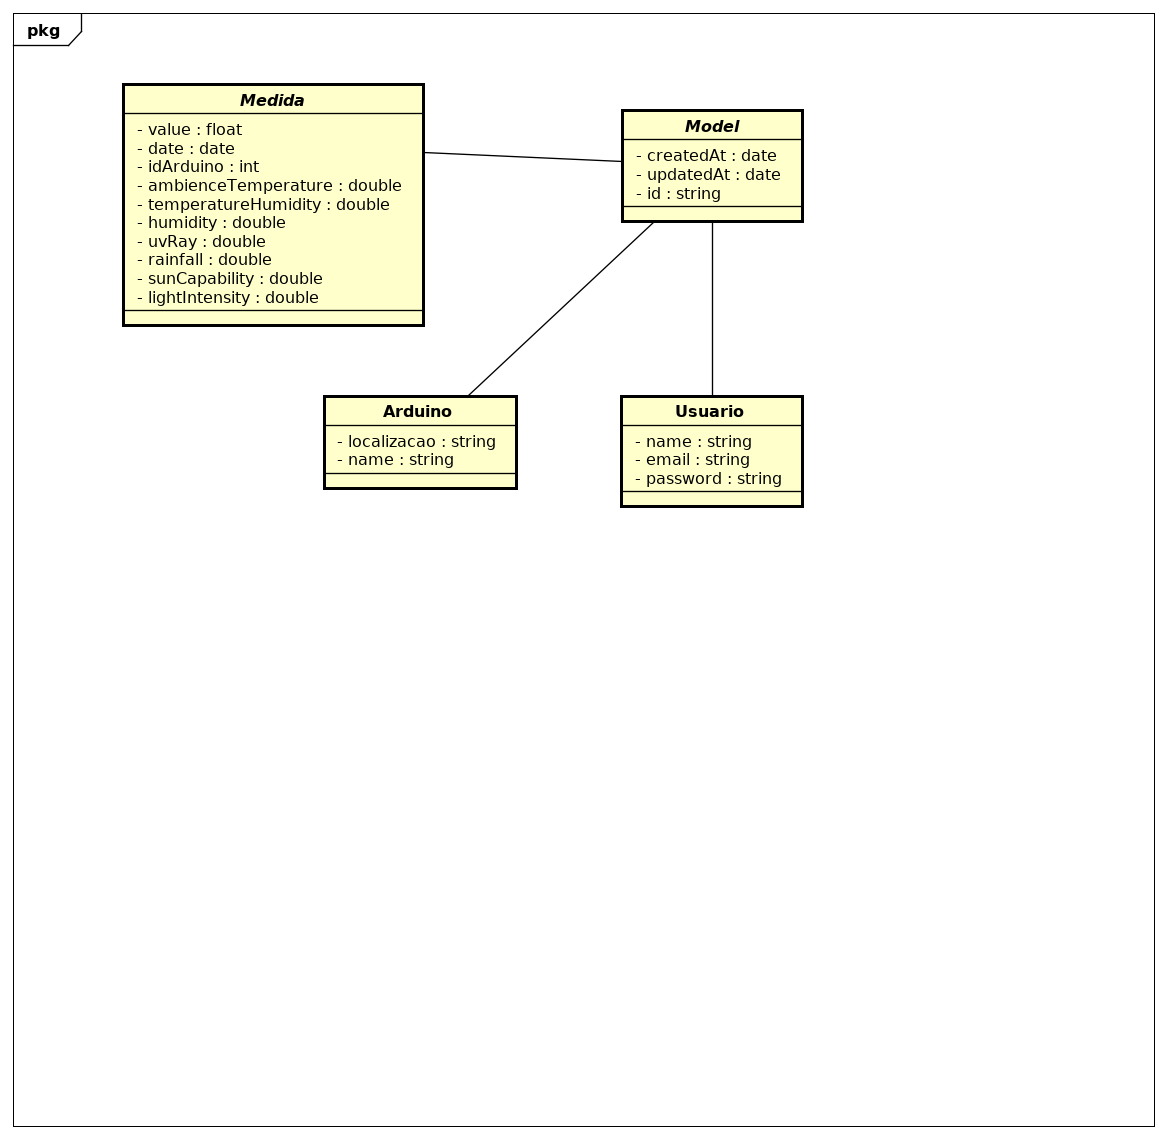
\includegraphics[scale=0.5]{diagrams/classe.png}
    \hfill
\end{figure}

\subsection{Diagrama de sequência}

Apresentação do diagrama de sequencia do projeto.

\begin{figure}[H]
    \label{figure_diagrama_sequencia}
    \centering
    \caption{Diagrama de sequência}
    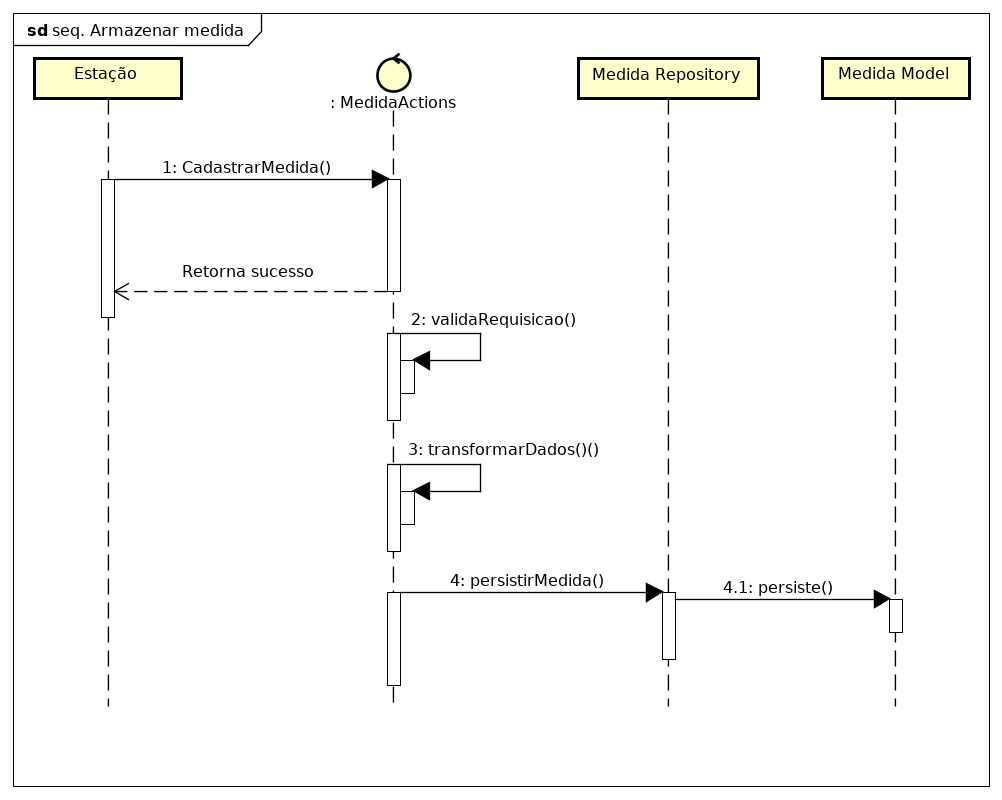
\includegraphics[scale=0.40]{diagrams/sequencia.png}
    \hfill
\end{figure}

Como descrito no diagrama de sequência representado na figura \ref{figure_diagrama_sequencia} a aplicação é composta por 3 principais camadas.

\subsubsection{Controlador}

Na camada de controle, os dados são recebidos e passam por uma básica validação através, porém não sofrem a interferência das regras de negócio.

Nessa camada, os dados são recebidos e retornados ao cliente, é uma interface de acesso a aplicação, geralmente, essa camada recebe objetos de requisições HTTP.

\subsubsection{Serviço}

Na camada de serviço as ações são os casos de uso, o caso de uso responsável por aquela ação trabalha, inserindo os dados através do repositório no banco de dados, e então, retorna as informações.

\subsubsection{Repositório}

Dentro da camada de repositório, são recebidos dados que, através de uma camada de infraestrutura são persistidos, retornando então, uma entidade.

\subsection{Diagrama de estado}

Apresentação dos estados de uma entidade de medida que foi capturada ao longo da interação com o sistema.

\begin{figure}[H]
    \label{figure_diagrama_estado}
    \centering
    \caption{Diagrama de estado}
    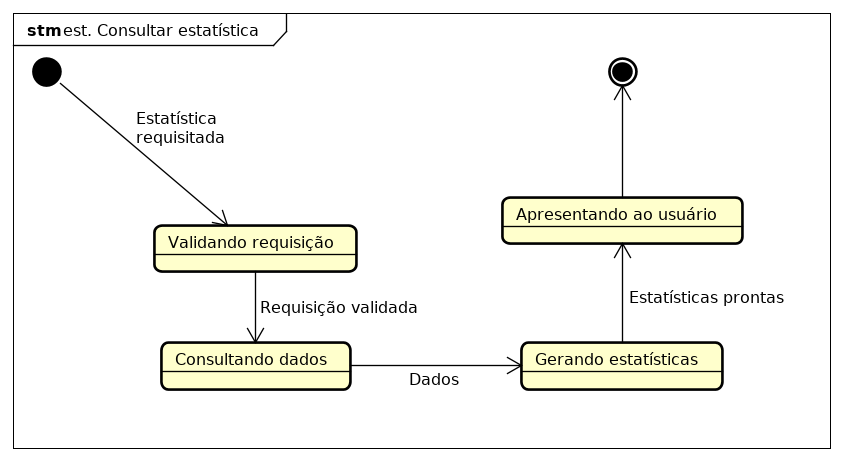
\includegraphics[scale=0.6]{diagrams/estado.png}
    \hfill
\end{figure}

Conforme descrito na figura \ref{figure_diagrama_estado} os estados durante o armazenamento de uma de uma medida são:

\subsubsection{Validando requisição}

A autenticação do arduino na API foi feita e a requisição HTTP para o armazenamento de uma medida foi feita até a API.
Nesse estado, a requisição está passando por uma validação básica, verificando os tipos e formato dos dados.

\subsubsection{Armazenando em banco de dados}

A medida é valida e está sendo armazenada no banco de dados, após, ela é retornada a camada de serviço.

\section{Arquitetura das estações meteorológicas}

Foi utilizado para a captura dos dados o microcontrolador arduino, que, com sensores conectados a sua porta serial, prepara os dados e envia uma string json contendo as medidas para o nodeMCU.
A placa serial nodeMCU é responsável por se conectar a internet através de Wifi e envia o json para a api.

\subsection{Sensores}

Os sensores do arduino, são ligados através da protoboard até o arduino, onde a captação é feita e as informações são tratadas, os dados são montados dentro de uma string JSON, que é enviada para o nodeMCU.

Não foi utilizada a biblioteca para a montagem da string JSON por conta da memória limitada do controlador.

\subsection{NodeMCU}

Na placa de WiFi NodeMCU, as informações são recebidas através da porta serial e o json recebido é enviado para a api.

\section{Arquitetura do software}
\label{sec:arquitetura_software}

A arquitetura da aplicação desenvolvida pode ser resumida em dados sendo capturados através de sensores conectados a um microcontrolador arduino, serão captadas as seguintes informações: temperatura, umidade do ar, temperatura em relação a umidade, porcentagem de chuva, radiação uv, intensidade luminosa e capacidade solar.

Dados esses, que serão enviados através de requisições HTTP para uma API, serão armazenadas em banco de dados e então, será feita uma análise estatística dessas informações.

A interface do usuário final com a aplicação, será feita através de uma aplicação web, onde os dados analisados serão disponibilizados e o usuário fará consultas a essas informações.

\subsection{Servidor}

TODO: ARQUITETURA DE SERVIDOR

\subsubsection{Implementação do servidor}

TODO: IMPLEMENTACAO DO SERVIDOR

\subsubsection{Banco de dados}

O banco de dados utilizado foi o MongoDB, um banco de dados não relacional, o desenho do banco de dados é controlado pela aplicação, que define quis campos devem ser indexados e como os dados devem se "relacionar", cada informação capturada fica armazenada dentro de uma coleção, utilizando o formato JSON.

A escolha de um banco de dados não relacional, foi motivada pela facilidade ao se trabalhar com esquemas maleaveis, podendo ter suas informações mutadas, deixando a cargo da aplicação a tomada de decisão.

O banco MongoDB foi escolhido pela sua facilidade ao trabalhar com escrita de dados concorrente, pois, as informações são, em primeiro instante processadas e armazenadas em cache, e já são retornadas para a aplicação, somente após, o MongoDB se encarrega de realizar a inserção dos dados em disco.

Com todas as vantagens do banco de dados, a aplicação tira vantagem, se beneficiando no que toca performance, disponibilidade e mutabilidade das informações.

\subsubsection{Tratamento dos dados}

Os dados foram exibidos da mesma forma que foram capturados, com exceção das informações de intensidade de luz, que foi invertida para melhor exibição no gráfico, e pela medida de nível de chuva, que além de invertida, foi transformada em porcentagem.

\subsubsection{Análise dos dados}

\subsubsubsection{Médias}

A média aplicada em cima dos dados, é separada por um intervalo de tempo, como exemplo, caso o usuário informe que o intervalo requisitado é de uma hora, os dados são agrupados por cada hora e então, uma média é aplicada nesses dados, exibindo as médias em intervalos de horas no gráfico.

\subsubsubsection{Mínimas e Máximas}

TODO: Mínimas e máximas

\subsubsection{Documentação da API}

Podemos conferir abaixo a documentação das rotas da API.

\begin{table}[H]
    \centering
    \caption{Descrição das rotas da API}
    \label{table_api_routes}
    \begin{tabular}{|l|l|l|}
    \hline
    \textbf{Método}  & \textbf{Rota}        & \textbf{Descrição}                           \\ \hline
    GET              & /arduino             & Lista os arduinos                            \\ \hline
    GET              & /arduino/:id         & Retorna os dados de um arduino               \\ \hline
    POST             & /arduino             & Cadastra um novo arduino                     \\ \hline
    POST, PATCH, PUT & /arduino/:id         & Atualiza os dados de um arduino              \\ \hline
    DELETE           & /arduino/:id         & Deleta um arduino e suas medidas capturadas  \\ \hline
    GET              & /user                & Lista os usuários                            \\ \hline
    GET              & /user/:id            & Retorna os dados de um usuário               \\ \hline
    POST             & /user                & Cadastra um novo usuário                     \\ \hline
    POST, PATCH, PUT & /user/:id            & Atualiza os dados de um usuário              \\ \hline
    DELETE           & /user/:id            & Deleta um usuário                            \\ \hline
    POST             & /user/login          & Recebe as credenciais e retorna o token      \\ \hline
    POST             & /measure             & Cadastra uma medida capturada                \\ \hline
    GET              & /statistic/:id       & Retorna as estatísticas de dados do arduino  \\ \hline
    \end{tabular}
\end{table}

\subsection{Cliente}

Foi utilizado para a construção do lado da interface do cliente a biblioteca react, que foi utilizada por sua alta performance na renderização de componentes no navegador, a interface aproveita da funcionalidade de renderização virtual da biblioteca para aumentar a performance e diminuir o custo computacional.

\subsubsection{Descrição das telas}

TODO: DESCRICAO DAS TELAS

% ----------------------------------------------------------
% Finaliza a parte no bookmark do PDF
% para que se inicie o bookmark na raiz
% e adiciona espaço de parte no Sumário
% ----------------------------------------------------------
\phantompart

\chapter{Conclusão}

TODO: Conclusão

\section{Resultados}

TODO: Resultados

\section{Projeções futuras}

TODO: Projeções futuras